\documentclass[10pt]{article}
\usepackage[left=2.5cm,right=2.5cm,top=2cm,bottom=2cm]{geometry}
% -------------------------------------------------------------------
\usepackage[english]{babel}
\usepackage[utf8]{inputenc}									
\usepackage[T1]{fontenc}										% 
% -------------------------------------------------------------------
\usepackage{amsmath,amsfonts,amssymb,amsthm,cancel,siunitx,
calculator,calc,mathtools,empheq,latexsym}
\usepackage[version=4]{mhchem}
\usepackage[official]{eurosym}
% -------------------------------------------------------------------
\usepackage{subcaption,epsfig,tikz,float}
\usepackage{xcolor}
\usepackage{booktabs,multicol,multirow,tabularx,array}
\usepackage{multicol}
\usepackage{lipsum}
\usepackage{csquotes}
\usepackage[super]{nth}
\usepackage[numbers]{natbib}
\usepackage{xurl}
\usepackage[breaklinks]{hyperref}
\urlstyle{same}
\hypersetup{
    colorlinks,
    breaklinks=true,
    linkcolor={black!50!black},
    citecolor={blue!50!blue},
    urlcolor={blue!80!blue}
}
	

% Commands
\newcommand*{\doi}[1]{\href{http://dx.doi.org/#1}{doi: #1}}

% Aliases
\let\autocite\cite

% -------------------------------------------------------------------
\setlength{\parindent}{0pt}
\setlength{\parskip}{5pt}
% \textheight 19.5cm
\columnsep .5cm
% -------------------------------------------------------------------
\title{\renewcommand{\baselinestretch}{1.17}\normalsize\bf%
\uppercase{The Role of Projects of Common Interest\\in Reaching European Energy Policy Targets}\\--- working title ---
}
% -------------------------------------------------------------------
% Authos
\author{%s
Bobby Xiong$^{1,*}$, Iegor Riepin$^{1}$, Tom Brown$^{1}$\\ 
}
\date{}
% -------------------------------------------------------------------

% GRAPHICS	
\graphicspath{
    {graphics/}
  }
\DeclareGraphicsExtensions{.pdf,.jpeg,.png,.jpg}


\begin{document}

\maketitle

\vspace{-1cm}

\begin{center}
{\footnotesize 
$^1$Technische Universität Berlin, Department of Digital Transformation in Energy Systems, Germany \\
$^*$Presenting author: \href{mailto:xiong@tu-berlin.de}{xiong@tu-berlin.de}
}\\
\smallskip
\footnotesize
\textbf{Tags}: energy system modelling, energy policy, infrastructure, resilience \\
\medskip
\textbf{\nth{43} International Energy Workshop --- relevant conference topics:}\\(1) Reaching net-zero emissions and climate neutrality \textbullet{} (2) Role of renewable energy in the energy transition \textbullet{} (3) Role of hydrogen, ammonia, e-fuels and e-methane in the energy transition \textbullet{} (4) Managing power system transitions --- integration of variable renewable energy and power-to-X \textbullet{} (5) Sectoral pathways for the energy transition --- transport, industry, and buildings \textbullet{} (6) Energy transition infrastructure --- assessment of infrastructure to enable the energy transition, including electrical transmission, storage, EV charging, and hydrogen distribution, CCS and CDR \textbullet{} (12) Climate resilience of energy systems \textbullet{} (13) Utilisation of scenarios by governments
\end{center}

% -------------------------------------------------------------------

\section*{Summary (max. 200 words)}

The European Union (EU) aims to achieve climate-neutrality by 2050, with ambitious 2030 targets, including a \SI{55}{\percent} reduction in greenhouse gas emissions, \SI{10}{Mt} p.a. of green \ce{H2} production, and \SI{50}{Mt} p.a. of \ce{CO2} sequestration. Projects of Common Interest (PCI) and Projects of Mutual Interest (PMI) provide cross-border infrastructure which support these goals.
Using the open-source, sector-coupled energy system model PyPSA-Eur, we assess the impact of PCI-PMI projects on the EU energy system, focusing on power, heat, transport, industry, and agriculture. We look into how a delay of such projects may impact reaching the EU's policy targets. While preliminary results for 2030 suggest that the policy targets can be achieved even without PCI-PMI projects, they bring additional benefits: i) \ce{H2} pipelines improve affordability and distribution of green \ce{H2} and kickstart the hydrogen economy, ii) \ce{CO2} transport projects connect major industrial emissions to offshore sequestration sites in the North Sea.
Next steps include incorporating all remaining PCI-PMI projects, i.e. hybrid interconnectors and \ce{CO2} shipping routes, as well as the assessment of long-term pathway effects towards 2050. Our findings underscore the interplay between cross-border cooperation, infrastructure investments, and policy targets in the European energy transition throughout all sectors.

\section*{Introduction and motivation}

On the pathway to a climate-neutral Europe by 2050, the European Union (EU) has set ambitious targets for 2030, three of the most prominent including a reduction of \SI{55}{\percent} in greenhouse gas emissions \autocite{europeancommissionFit55Delivering2021}, \SI{10}{Mt} p.a. green \ce{H2} production \autocite{europeancommissionREPowerEUPlanCommunication2022}, and \SI{50}{Mt} p.a. \ce{CO2} sequestration \autocite{europeanparliamentRegulationEU20242024}. 

To support reaching these targets, the EU has identified a list of Projects of Common Interest (PCI) which are key cross-border infrastructure projects that link the energy systems of EU countries, ranging from storages, over transmission lines to pipelines and carbon sinks \autocite{europeancommissionCommissionDelegatedRegulation2023}. Projects of Mutual Interest (PMI) further include cooperations with countries outside the EU, such as Norway or the United Kingdom. In order for projects to be eligible for PCI-PMI status, their potential benefits need to outweigh their costs \autocite{europeancommissionCommissionDelegatedRegulation2023}. Given the political and lighthouse character, these projects are highly likely to be implemented. However, any large infrastructure project, including PCI-PMI projects, are commonly facing delays due to permitting, financing, procurement bottlenecks, etc. \autocite{acerConsolidatedReportProgress2023}.

\paragraph{Research questions} From the ambitious policy targets and the nature of PCI-PMI projects, we derive the following key research questions:

\begin{enumerate}
    \item At what cost do we stick to reaching the EU policy targets?
    \item How does a delay of PCI-PMI projects affect the system, its costs, and the ability to reach the EU policy targets?
    \item What is the impact of missing the EU 2030 policy targets for \ce{CO2} sequestration and \ce{H2} production?
 \end{enumerate}

\section*{Methodology}

We use the open-source, sector-coupled energy system model PyPSA-Eur \cite{neumannPotentialRoleHydrogen2023,frysztackiComparisonClusteringMethods2022,glaumOffshorePowerHydrogen2024,horschPyPSAEurOpenOptimisation2018} to optimise investment into generation, storage, and transmission infrastructure (including electricity, natural gas, hydrogen, \ce{CO2}, and Power-to-X conversion) as well as operation/dispatch. The model is spatially and temporally highly resolved and covers the entire European continent, including stocks of existing power plants \autocite{gotzensPerformingEnergyModelling2019}, renewable potentials, and availability time series \autocite{hofmannAtliteLightweightPython2021}. It covers today's high-voltage transmission grid (AC \SI{220}{kV} to \SI{750}{kV} and DC \SI{150}{kV} upwards) \autocite{xiongModellingHighVoltageGrid2024}.

\paragraph{Feature implementation} By accessing the REST API of the PCI-PMI Transparency Platform \autocite{europeancommissionPCIPMITransparencyPlatform2024} and associated public project sheets provided by the European Commission, we implement the PCI-PMI projects into the PyPSA-Eur model to assess their impact in the power, heat, transport, industry, feedstock, and agriculture sector. Our implementation can adapt to the needs and configuration of the model, including selected technologies, geographical and temporal resolution, as well as the level of sector-coupling. An overview of the implemented PCI-PMI projects is shown in Figure \ref{fig:pci_pmi_projects_map}.

\begin{figure}[!htbp]
    \centering
    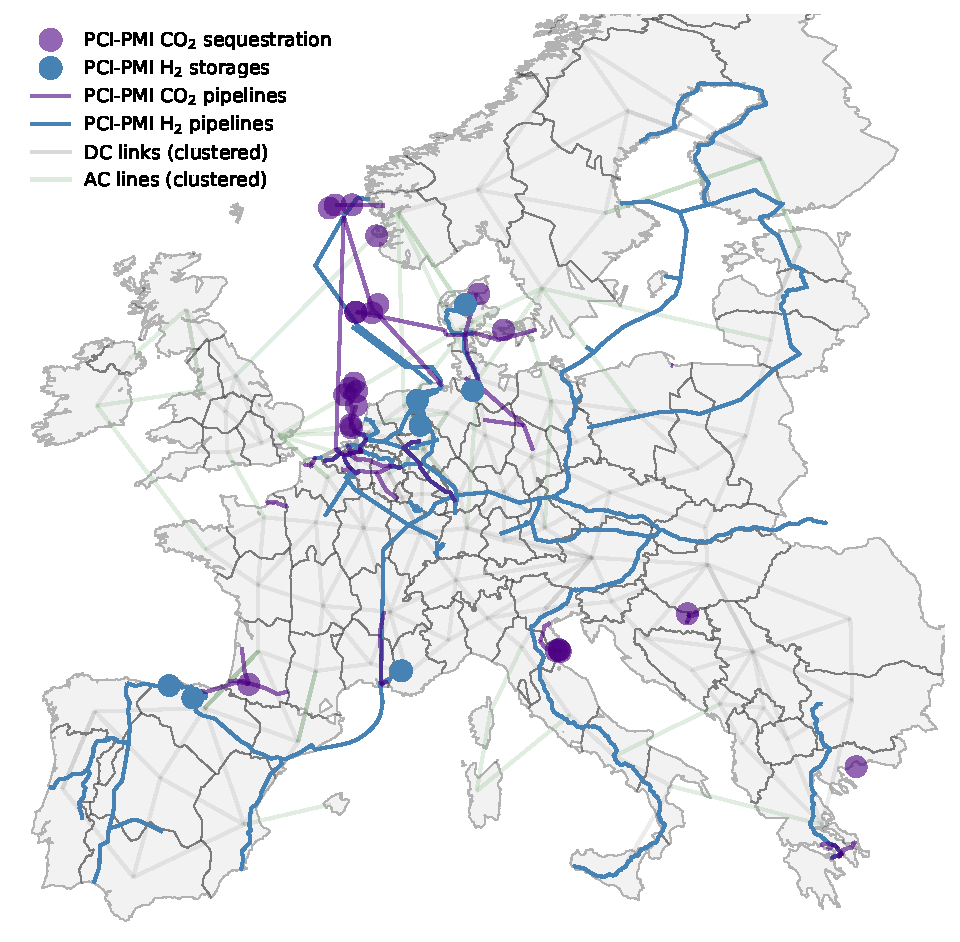
\includegraphics[width=0.55\textwidth]{pci_pmi_projects_map}
    \caption{PCI-PMI projects implemented in the PyPSA-Eur model as of the date of submission. Own illustration based on data from the European Commission \autocite{europeancommissionPCIPMITransparencyPlatform2024}.}
    \label{fig:pci_pmi_projects_map}
\end{figure}

\paragraph{Scenario setup} As of the date of submission, we model three key scenarios for the target year 2030 which will set the base year for pathways towards 2050: a `Base' scenario in which policy targets are achieved and all projects are commissioned on time as well as two PCI-PMI delay scenarios `A' and `B'. Table \ref{tab:scenarios} gives an overview of the scenarios' key assumptions and their differences. Depending on the scenario, we formulate and activate additional constraints to ensure the fulfilment of the EU policy targets.

\begin{table}[!htbp]
    \centering
    \caption{Initial scenario setup. Own illustration.}
    \begin{tabular}{lccc}
        \toprule
        Assumption \textbackslash{} Scenario & Base & A. All targets & B. Emission target only \\
        \midrule
        PCI-PMI projects & on time & delayed & delayed \\
        \midrule
        \ce{CO2} emission target & \SI{-55}{\percent}/\SI{2}{Gt} p.a. & \SI{-55}{\percent}/\SI{2}{Gt} p.a. & \SI{-55}{\percent}/\SI{2}{Gt} p.a. \\
        \ce{CO2} sequestration target & \SI{50}{Mt} p.a. & \SI{50}{Mt} p.a. & --- \\
        \ce{H2} target & \SI{10}{Mt} p.a. & \SI{10}{Mt} p.a. & --- \\
        \midrule
        \ce{CO2} sequestration sites & PCI-PMI & endogeneous & endogeneous \\
        \ce{CO2} pipelines & PCI-PMI + endogen. expansion & --- & --- \\
        \ce{H2} storage & PCI-PMI & endogeneous & endogeneous \\
        \ce{H2} pipelines & PCI-PMI +  endogen. expansion & --- & --- \\
        AC and DC transmission & PCI-PMI & --- & --- \\
        \bottomrule
    \end{tabular}
    \label{tab:scenarios}
\end{table}

\paragraph{Solving} We solve all scenarios by minimising total system costs, resolving 34 countries to 90 buses at 3-hourly temporal resolution.

\section*{Results (preliminary)}
First results for the modelling year 2030 show that reaching the EU's 2030 \ce{H2} production and \ce{CO2} sequestration targets translates into around 20 bn. \euro{} p.a. in total system costs for all included sectors, with or without PCI-PMI infrastructure projects (see Figure \ref{fig:system_costs}).

\begin{figure}[!htbp]
    \centering
    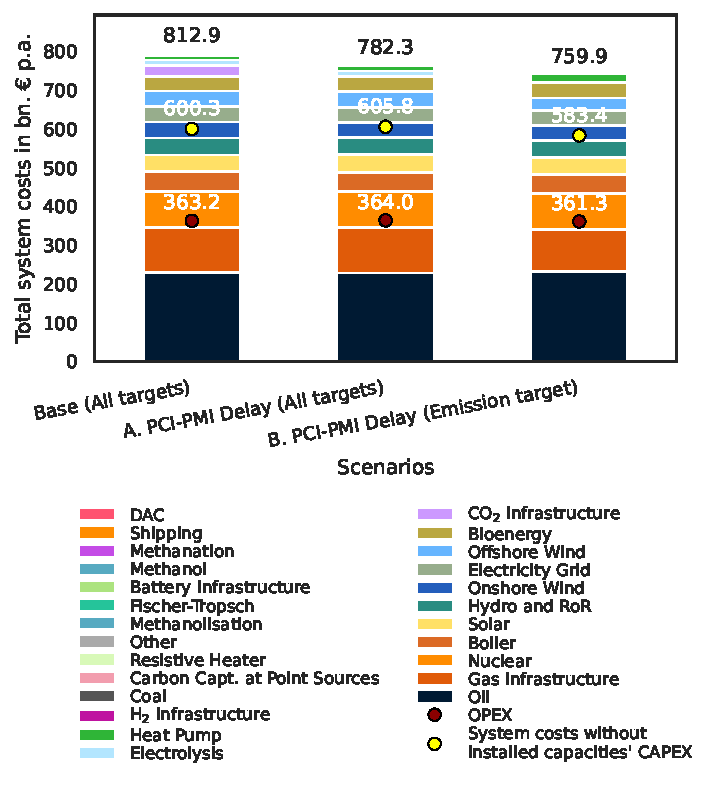
\includegraphics[width=1\textwidth]{system_costs}
    \caption{Results --- Total system costs by technology and infrastructure. Own illustration.}
    \label{fig:system_costs}
\end{figure}

By omitting an \ce{H2} target, almost no electrolysers are installed. Around \SI{8}{Mt} are still produced to cover industrial \ce{H2} and methanol (primarily shipping) demand. However, this demand is met by decentral steam methane reforming instead of electrolysers. 
Figure \ref{fig:balance_maps} shows the regional distribution of the \ce{H2} and \ce{CO2} value chain in the Base scenario. Note that for the specific year of 2030, a disconnect in \ce{H2} infrastructure between central and southeastern Europe can be observed, due to the delay in commissioning of the project connecting the two networks. Utilisation of \ce{H2} pipelines vary strongly across the PCI-PMI projects. In most of the times, pipelines serve the purpose of transporting \ce{H2} in a single direction only, i.e. from high renewable potential regions to \ce{H2} consumption sites, where it serves as a precursor for methanolisation or direct use in industry and shipping (see Figure \ref{fig:balance_map_h2}). Prominent PCI-PMI projects with particularly high full-load hours include P9.9.2 \textit{Hydrogen Interconnector Denmark-Germany} (\SI{6937}{h}) and P11.2  \textit{Nordic-Baltic Hydrogen Corridor} (\SI{2295}{h}), followed by projects connecting major steel-industrial and chemical sites of Germany (southwest) with Belgium (P9.4 \textit{H2ercules West}, \SI{1634}{h}), the Netherlands (P9.6 \textit{Netherlands National Hydrogen Backbone}, \SI{1967}{h} and P9.7.3 \textit{Delta Rhine Corridor H2}, \SI{1510}{h}), and France (P9.2.2 \textit{MosaHYyc}, \SI{4662}{h}).

\begin{figure}[h!]
    \centering
    \begin{subfigure}[t]{0.495\textwidth} % [t] aligns at the top
        \vspace{0pt}
        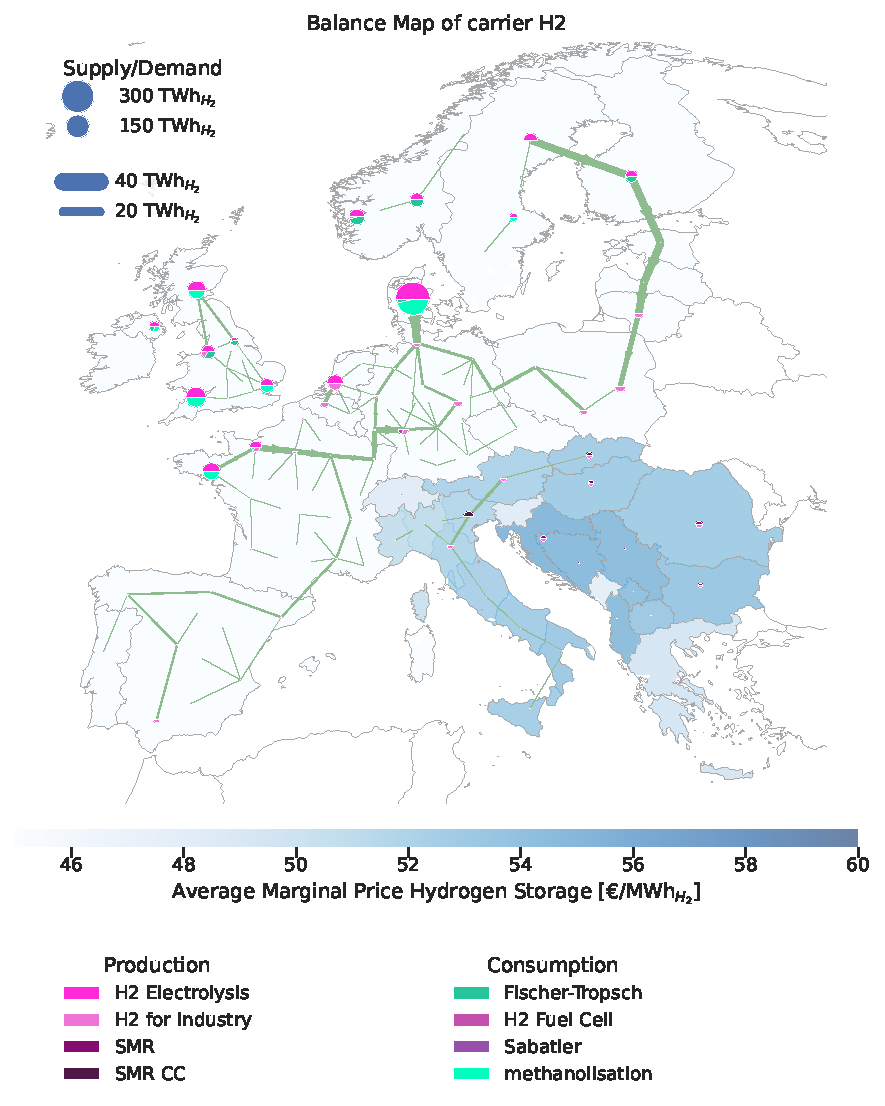
\includegraphics[width=\textwidth]{balance_map_h2} % Replace with your image
        \caption{\ce{H2} regional balances and flows.}
        \label{fig:balance_map_h2}
    \end{subfigure}
    \hfill
    \begin{subfigure}[t]{0.495\textwidth} % [t] aligns at the top
        \vspace{0pt}
        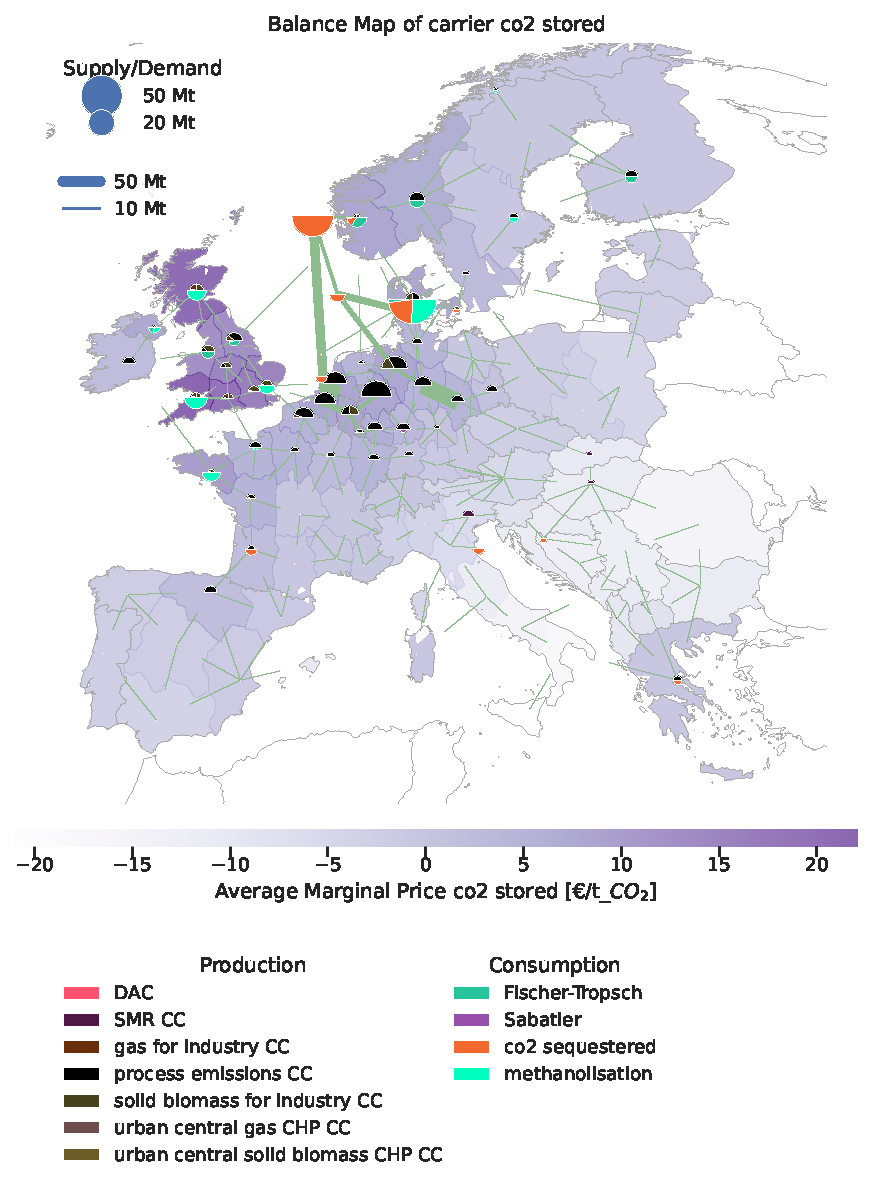
\includegraphics[width=\textwidth]{balance_map_co2} % Replace with your image
        \caption{\ce{CO2} regional balances and flows.}
        \label{fig:balance_map_co2}
    \end{subfigure}
    \caption{Results --- Regional distribution of \ce{H2} and \ce{CO2} production, utilisation, storage, and transport in the Base scenario. Own illustration.}
    \label{fig:balance_maps}
\end{figure}

Figure \ref{fig:balance_map_co2} shows the regional distribution of \ce{CO2} production, utilisation, storage, and transport in the Base scenario. PCI project P13.8 \textit{EU2NSEA} connects \ce{CO2} from process emissions in Germany, Belgium and the Netherlands to major geological sequestration sinks close to the Norwegian shore \textit{Smeaheia} and \textit{Luna} with an annual injection potential of \SI{20}{Mt} p.a. and {5}{Mt} p.a., respectively. 
Without specifying a \ce{CO2} sequestration target, the system still collects around \SI{21}{Mt} of \ce{CO2} p.a. primarily from process emissions in the industry sector and sequesters it in carbon sinks near industrial sites where a sequestration potential is identified \autocite{hofmannH2CO2Network2024}. As no pipeline infrastructure is built in these scenarios, the chosen locations differ in the delay scenarios --- this can be observed for regions near the coast, such as the United Kingdom and Norway.

\section*{Conclusion (preliminary)}
We conclude that while all three EU policy targets for 2030 can be achieved without PCI-PMI infrastructure, they bring additional benefits: i) \ce{H2} pipelines projects help distribute more affordable green H$_2$ from northern and south-western Europe to high-demand regions in central Europe; ii) \ce{CO2} transport and storage projects help decarbonising the industry by connecting major industrial sites and their process emissions to offshore sequestration sites in the North Sea (Denmark, Norway, and the Netherlands).

\paragraph{Research outlook} Next steps include the implementation of remaining PCI-PMI projects, such as hybrid offshore interconnectors (energy islands), electricity storages, and \ce{CO2} shipping routes. To evaluate the long-term value of PCI-PMI projects in a sector-coupled European energy system, we will model pathway dependencies towards 2050. We will also assess the sensitivity of the infrastructure to technology-specific build-out rates.

% % -----------------------------

\bibliographystyle{plainnat}
\bibliography{references.bib}

\end{document}